\chapter{Simulation of Reconstruction Algorithm}
This chapter will describe how the system can be mathematically modelled and how the mask for the lensless imager was designed. As mentioned in the previous chapter the system can be modelled as 
\begin{equation}
\label{eq:conv2}
y = \phi * x + e ;
\end{equation}
Ignoring the noise and converting the equation to fourier domain, the equation \ref{eq:conv2} can be re-written as
\begin{equation}
\label{eq:conv3}
F(y) = F(\phi)F(x)
\end{equation}
\begin{equation}
\label{eq:conv3}
F(x) = \frac{F(y)}{F(\phi)}
\end{equation}
\begin{equation}
\label{eq:conv4}
x = F^{-1}(\frac{F(y)}{F(\phi)})
\end{equation}
Equation \ref{eq:conv4} is the simplest possible computational inversion of the scene from the sensor. This method has also been used in \cite{Toeplitz}. As mentioned in the previous chapter, there are two types of masks that can be used for the purpose of encoding the scene onto the mask, namely separable and non-separable mask. MATLAB has been used for the purpose of simulating the algorithms. In this chapter, we would simulate two types of mask patterns, namely separable and non-separable mask patterns. A separable mask pattern is one in which the mask matrix $\phi$ can be expressed in-terms of two sub- matrices:
\begin{equation}
\phi = \phi_L * \phi_R
\end{equation}
Both $\phi_L$ and $\phi_R$ are doubly-toeplitz mask. The mathematical model is also changed as described by the equation \ref{eq:separable}. A non-separable mask is one which does not follow this property and follows equation \ref{eq:conv2}.

\section{Simulation of a non-separable mask}
The non-separable mask simulation was carried out as shown in Figure \ref{fig:non_sep_sim}. Due to the inherent ill-posed mathematics involved in imaging extended scenes, a regularization term is added to the inversion process and we get equation \ref{eq:conv5}. This kind of regularization is called Tikhonov regularization and it regularizes the inversion and controls the effects of noise\cite{Toeplitz}. The same regularization is also used in previous studies\cite{Toeplitz}.

\begin{equation}
\label{eq:conv5}
x = F^{-1}(\frac{F(y)}{F(\phi)+k})
\end{equation}
\begin{figure}[ht]
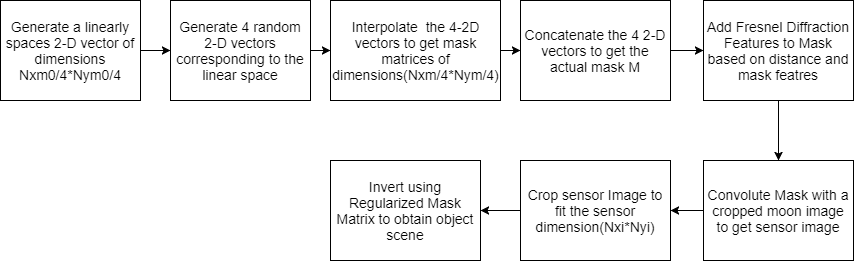
\includegraphics[width=\linewidth]{pics/non_sep_sim_flow}
\caption{Simulation-Flow non-separable mask}
\label{fig:non_sep_sim}
\end{figure}

In order to start with the mathematical modeling process and to imitate the sensor data and reconstruction, a reference image is needed. For that, it was decided to use the full moon image captured by the Apollo 11 space craft\cite{MoonImage}. Since the satellite is going to be pointing towards astronomical objects like the earth, moon, it was decided to crop out a portion of the full moon image as the main purpose of the satellite would be to image specific portions of the earth. The simulation is done under the assumption that the camera is enclosed in a box-like structure and light from a specific region of the earth/moon would reach it and the sensor size is finite. The image was converted to gray and scaled down from 0 to 1 and is displayed in the \texttt{bone} colormap format available in MATLAB as the colormap would display the minute variations in the reconstructed image. This is illustrated in Figure \ref{fig:moon_image}. The simulation is performed with and without diffraction and analyzed. The mask used for simulation is shown in Figure \ref{fig:non_sep_sim}.
\begin{figure}[ht]
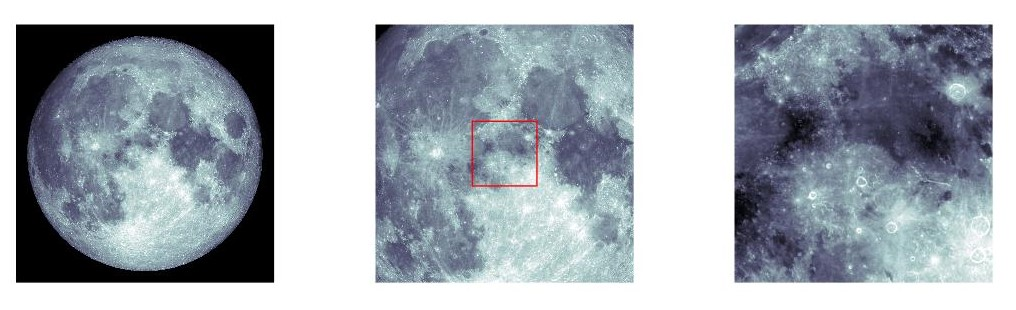
\includegraphics[scale = 0.50]{pics/MoonImagePortion}
\caption{The first image is the original image of the moon as taken by Apollo 11 spacecraft. The second image indicates the cropped region and the third image indicates the region that is used for the simulation.}
\label{fig:moon_image}
\end{figure}
The simulation parameters are shown in Table \ref{tbl:sim_parameters}. The reconstruction error is given by the equation \ref{eq:psnr}. $O_{guess}$ indicates the reconstruction and $O$ represents the original object. Fresnel diffraction features are added to the mask since the distance between the mask and the sensor lies in the Fresnel diffraction region and the Fresnel number for the mask is less than  1. The Fresnel diffraction modeling is described in the appendix section of the report.Diffraction causes the mask to become non-binary.
\begin{equation}
PSNR = 20log(\frac{N*max(O)}{MSE})
\label{eq:psnr}
\end{equation}
where 
\begin{equation}
MSE = \frac{1}{mn}\sum_{i=1}^{i=N}\sum_{j=1}^{j=N}[O(i,j) - O_{guess}(i,j)]^2
\end{equation}

\begin{table}
\caption{Simulation Parameters}
\begin{center}
\begin{tabular}{ |c|c| }
\hline
Pixel Size & 2.2$\mu m$ * 2.2$\mu m$\\
\hline
Sensor Size & 512 * 512 pixels\\
\hline     
Mask Size & 1024 * 1024 pixels\\
\hline 
Mask Sensor Distance & 5 millimeters \\
\hline 
\texttt{Nxm0, Nym0} & 256, 256\\
\hline
\end{tabular}
\label{tbl:sim_parameters}
\end{center}
\end{table}

\begin{figure}[ht]
\centering
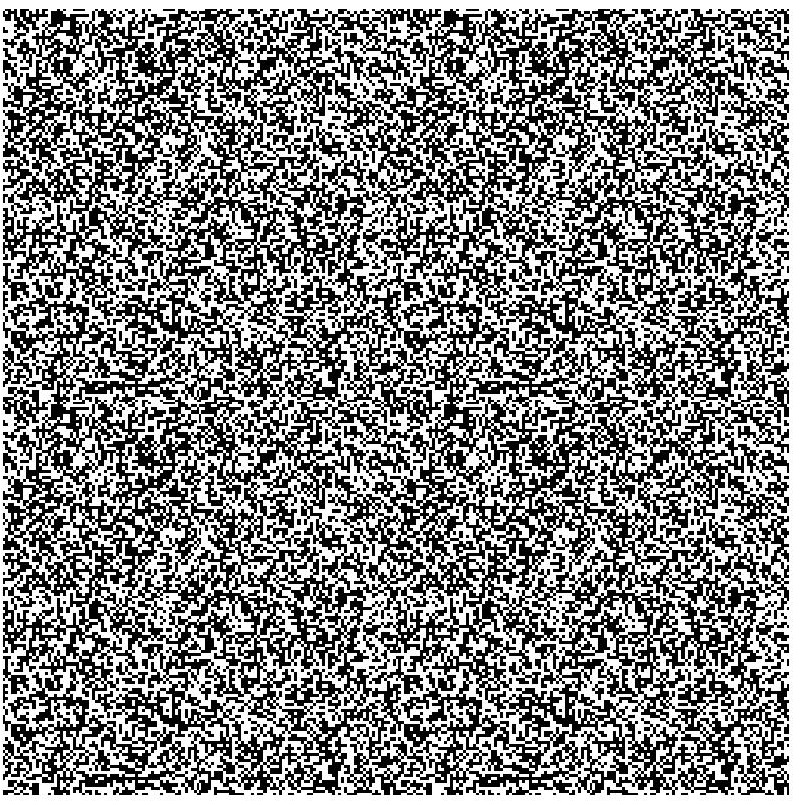
\includegraphics[scale = 0.250]{pics/non_separable_mask}
\caption{Non-separable mask used for simulation}
\label{fig:non_sep_sim}
\end{figure}

\begin{figure}[ht]
\centering
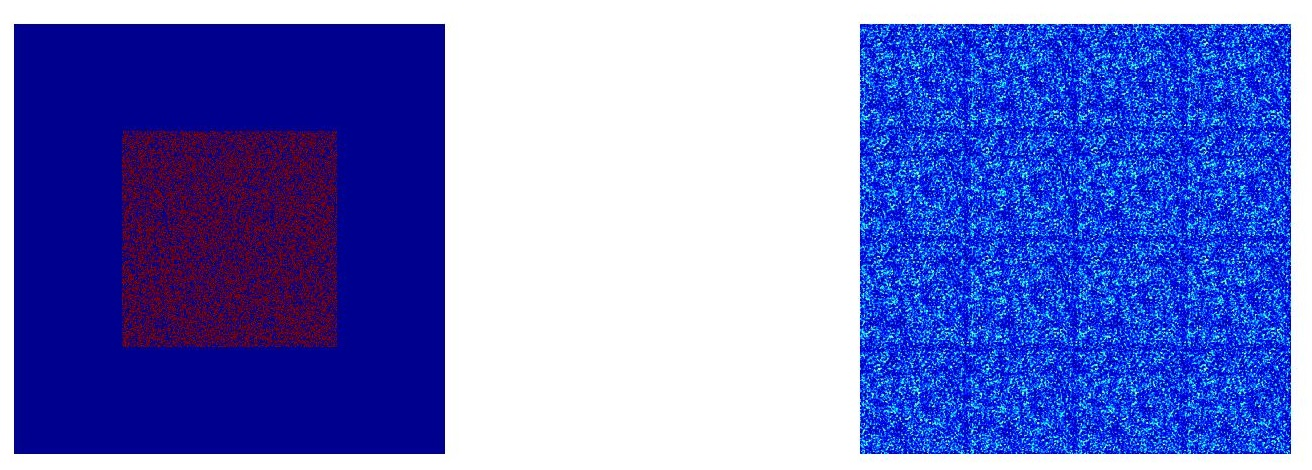
\includegraphics[width = \textwidth]{pics/non_sep_diffracted_mask}
\caption{The mask image on the left indicates undiffracted mask and the mask on the right indicates the diffracted non-separable mask}
\label{fig:non_sep_sim_diff}
\end{figure}

\begin{figure}[ht]
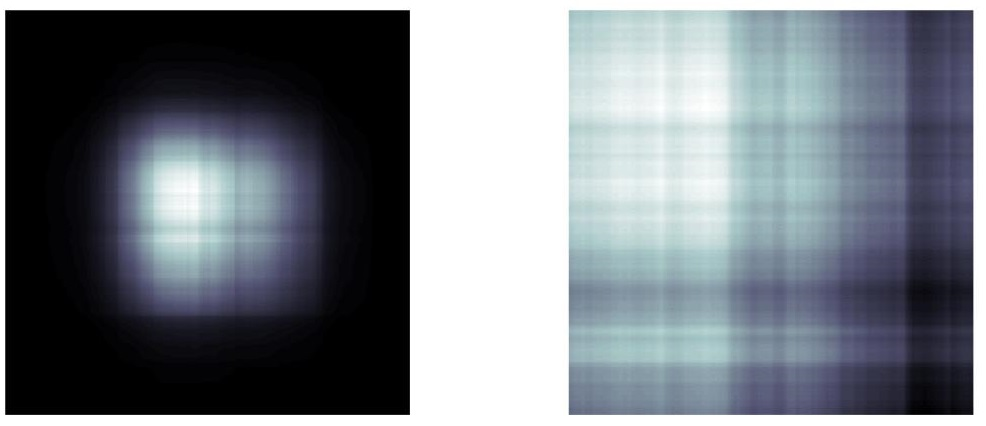
\includegraphics[scale = 0.50]{pics/sensorCropped}
\caption{The first image indicates the sensor image if the sensor plane was infinite. The second image indicates the cropped sensor image that would be formed on an actual finite sensor size(cropped).}
\label{fig:moon_image}
\end{figure}
The reconstructions obtained using equation \ref{eq:conv5} is shown in Figure \ref{fig:rec_non_sep}. It can be seen from the figure that we have successful reconstructions using equation \ref{eq:conv5}. The value of $k $ was set to 0.01.
However, when the diffracted mask is modeled for the sensor image, the reconstruction fails. This is the reason why we need to go for the separable mask as this mask is not resistant to diffraction effects. 
  \begin{figure}[ht]
    \centering
    \begin{subfigure}{0.5\textwidth}
    \centering
        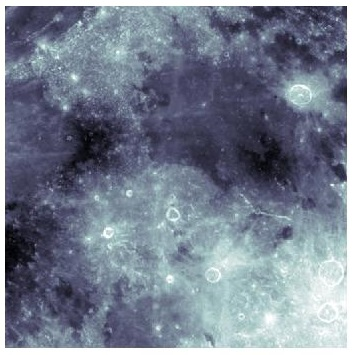
\includegraphics[scale = 0.5]{pics/rec_non_sep}
    
    \end{subfigure}%
    \begin{subfigure}{0.5\textwidth}
    \centering
        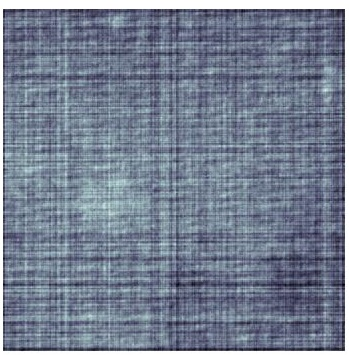
\includegraphics[scale= 0.5]{pics/rec_non_sep_diff}
    \end{subfigure}
    \caption{the figure shows the reconstruction with and without fresnel diffraction effects for a non-separable mask using equation \ref{eq:conv5}. We are able to obtain PSNR = 57.85 without diffraction effects. However, the reconstruction with the mask fails when diffraction effects are incorporated into the mask. }
    \label{fig:rec_non_sep}
    \end{figure}
    
    
\section{Simulation of a separable mask}
As we saw in the previous section, a non-separable mask cannot be used for our application in the visible light region as the visible light spectrum contains significant diffraction effects. We can improve the solution since a separable mask follows the equation \ref{eq:separable}. The same improved solution has been used in \cite{Toeplitz}. We can express \ref{eq:separable} as shown in equation \ref{eq:sep_sq}.
\begin{equation}
M_{A}^TIsM_{B} = (M_{A}^TM_{A})O(M_{B}^TM_B)^T 
\label{eq:sep_sq}
\end{equation} 
We multiply the left and right system matrices to obtain square symmetric matrices. The problem is that they are not invertible, due to the presence of zero eigenvalues. So, the parameters $\alpha_A$ and $\alpha_B$ to remove the zero eigenvalues and make them invertible. The final solution will be given by the equation \ref{eq:sep_final}.
\begin{equation}
O_{Guess} = (M_{A}^TM_A + \alpha_{A}^21_{R_{O}})^{-1}M_{A}^TIM_{B}(M_{B}^TM_B + \alpha_{B}^21_{C_{O}})^{-1}
\label{eq:sep_final}
\end{equation}
One more advantage of using the separable mask is the reduced amount of computation needed compared to the non-separable mask. The number of computations for a non-separable mask will be given by the equation \ref{eq:non_sep_comp}. For a megapixel image, this would translate to $10^{18}$.
\begin{equation}
N_{operations} \propto (r_O*c_O)^3
\label{eq:non_sep_comp}
\end{equation}

\begin{table}[ht]
\caption{Table indicating the rows and columns used for simulation}
\label{tbl:comp_sep}
\begin{center}
\begin{tabular}{ |c|c|c| }
\hline
Matrix & Rows & Columns \\
\hline
Mask Size & $r_M$ & $c_M$\\
\hline
Image on Sensor & $r_I$ & $c_I$\\
\hline
Object Area contributing &  $r_O = r_M + r_I - 1$ & $c_O = c_M + c_I - 1$\\
\hline
Left Toeplitz Mask & $r_{I}$ & $r_{O}$\\
\hline
Right Toeplitz matrix & $c_{I}$ & $c_{O}$\\
\hline
\end{tabular}
\end{center}
\end{table}


For a separable mask, however, the number of computation is drastically reduced because the size of the left and right system matrices is reduced to $(R_I*R_O)$ and $(C_I*C_O)$ from multiplying the entire object matrix of size $r_O*c_O$. This would come to around $2*10^9$ operations.This can also be observed in the simulation and it takes an extremely long amount of time to complete a non-separable matrix. The size of different matrices used in the simulation is shown in Table \ref{tbl:comp_sep}.

\begin{equation}
N_{operations} \propto [(r_I*r_O)^3 + (c_I*c_O)^3] 
\label{eq:sep_comp}
\end{equation}

The separable mask simulation was carried out as shown in Figure \ref{fig:sep_sim}. It is possible to generate different types of Toeplitz mask by simply changing the simulation variable \texttt{Nxm0}. These masks follow the same property and offer the same amount of reconstruction in the simulation. By changing \texttt{Nxm0}, the base vector that is used for interpolating to et the bigger mask changes. This lead to different masks being generated. The shape of the mask is simpler when we use a smaller \texttt{Nxm0} as a very small vector is used for interpolation to get a bigger mask. The transmittance of the masks varies between 20 to 25 percent. The different masks obtained by changing \texttt{Nxm0} is shown in Figure \ref{fig:sep_mask_multi}. By changing the \texttt{Nxm0}, we can basically change the feature size of the mask. A lower \texttt{Nxm0} generates a mask where the subsequent binary value comes at a greater distance than the one with a larger \texttt{Nxm0}. It can be seen from figure \ref{fig:sep_sim} that there as an additional step involved in the simulation process of separable masks which is the rank-1 estimation of diffracted matrices. In this step, we perform Singular Value Decomposition(SVD) on the diffracted matrices to obtain $M_x$ and $M_y$. Now let us see what is singular value decomposition. Singular value decomposition is a mathematical tool that would enable us to express any matrix of the form $M_{ \times n}$ in the form given by equation \ref{eq:svd_1}\cite{svd}. 

\begin{equation}
\label{eq:svd_1}
M_{m \times n} = U_{m \times r}S_{r\times r}(V_{n \times r})^T
\end{equation}
where $r$ represents the rank of the matrix $M$ , $m$ and $n$ denote the size of the matrix respectively. We can estimate the rank-1 estimation of a matrix by taking the first row and column of $U$ and $V$ and multiplying them as shown in equation \label{eq:svd_2}.

\begin{equation}
\label{eq:svd_2}
M_{1} = U_{1}S_1(V_{1})^T
\end{equation}
One of the main advantages of using a doubly Toeplitz mask is that it is decomposable into a single rank matrix with and without the effects of diffraction. The other rank-components are negligible even in the presence of diffraction. This is an important property that must be kept in mind which will be used for various experimental purposes.  In the simulation, we use SVD on the diffracted mask, take the rank-1 estimate of the mask. The $U_1$ and $V_1$ will represent the left and right system matrix of the refracted mask. The obtained single dimensional $U_1$ and $V_1$ of the doubly Toeplitz mask will be converted into Toeplitz matrices and inverted using equation \ref{eq:sep_final}. The decomposition of the diffracted and non-diffracted separable mask into a 1-rank matrix(with other components negligible) was also verified in the simulations.
The difference between diffracted and non-diffracted separable mask is shown in Figure \ref{fig:diff_separable}.
\begin{figure}[ht]
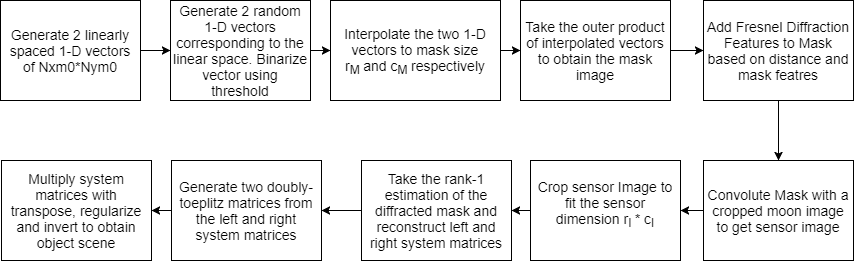
\includegraphics[width=\linewidth]{pics/sep_mask_sim_flow}
\caption{Simulation-Flow separable mask}
\label{fig:sep_sim}
\end{figure}
  \begin{figure}[ht]
    \centering
    \begin{subfigure}{0.5\textwidth}
    \centering
        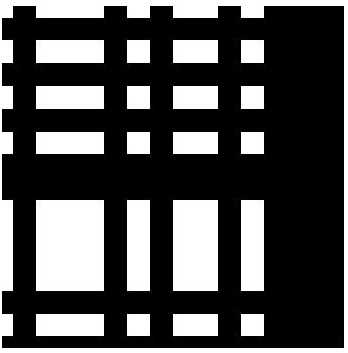
\includegraphics[width=0.5\linewidth]{pics/mask_16}
        \caption{\texttt{Nxm0} = 16}
        \label{fig:mask-16}
    \end{subfigure}%
    \begin{subfigure}{0.5\textwidth}
    \centering
        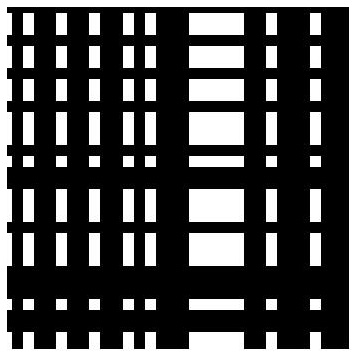
\includegraphics[width=0.5\linewidth]{pics/mask_32}
        \caption{\texttt{Nxm0} = 32}
        \label{fig:mask-32}
    \end{subfigure}
    
    \begin{subfigure}{0.5\textwidth}
    \centering
        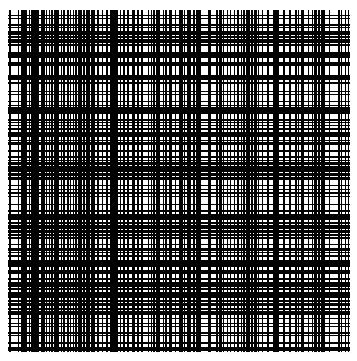
\includegraphics[width=0.5\linewidth]{pics/mask_256}
        \caption{\texttt{Nxm0} = 256}
        \label{fig:mask-256}
    \end{subfigure}%     
    \caption{Different separable masks generated with different \texttt{Nxm0}}
    \label{fig:sep_mask_multi}
    \end{figure}

\begin{figure}[ht]
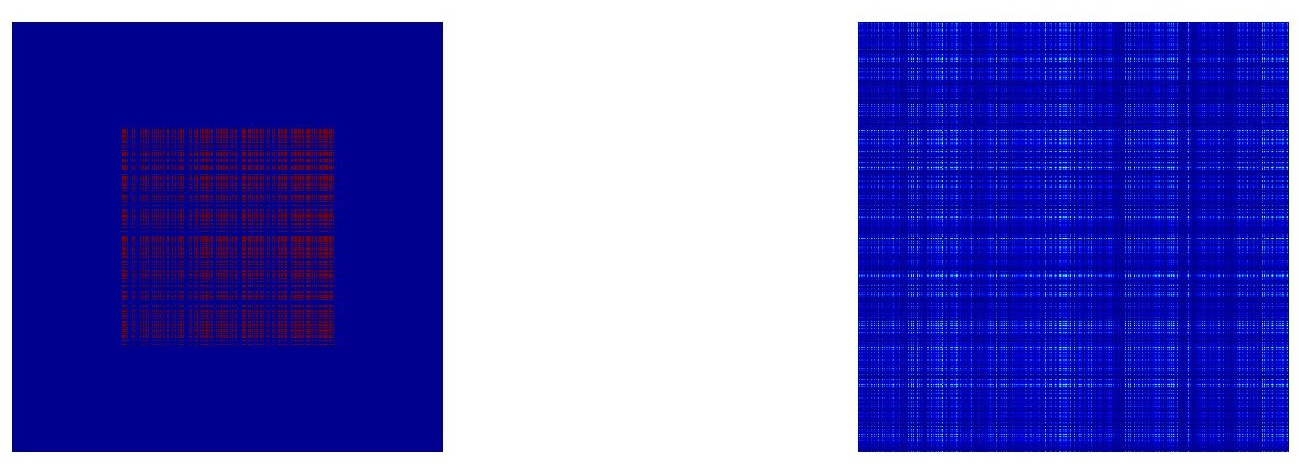
\includegraphics[width=\linewidth]{pics/diffracted_mask}
\caption{The mask image on the left indicates undiffracted mask and the mask on the right indicates the diffracted separable mask}
\label{fig:diff_separable}
\end{figure}

It can be seen from Figure \ref{fig:rec_sep} that even in the presence of diffraction it would be possible to obtain reconstructions using equation \ref{eq:sep_final} by using a separable mask, unlike a non-separable mask which fails to provide any reconstruction in the presence of diffraction effects. 
  \begin{figure}[ht]
    \centering
    \begin{subfigure}{0.5\textwidth}
    \centering
        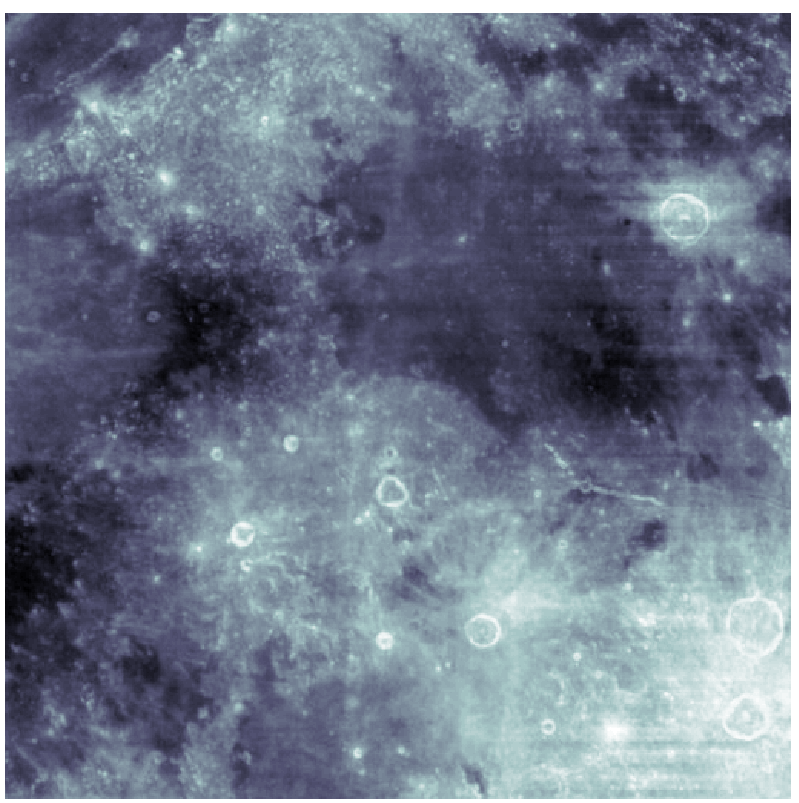
\includegraphics[scale = 0.25]{pics/sep_mask_rec}
    \end{subfigure}%
    \begin{subfigure}{0.5\textwidth}
    \hspace{4cm}    
    \centering
        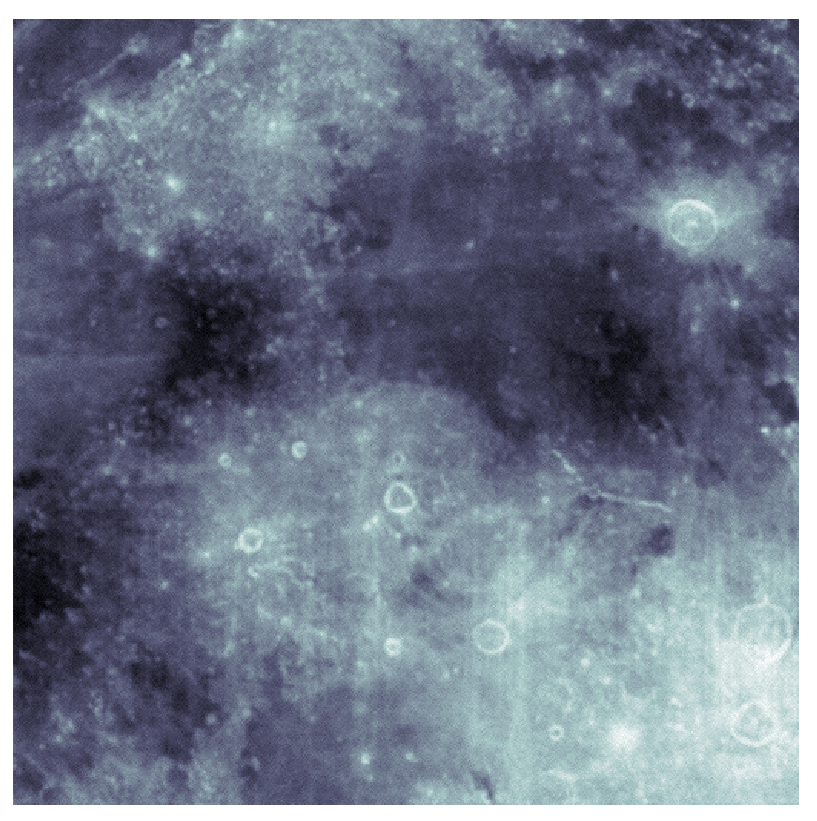
\includegraphics[scale= 0.25]{pics/sep_mask_rec_diff}
    \end{subfigure}
    \caption{The figure shows the reconstruction with and without fresnel diffraction effects for a separable mask using equation \ref{eq:sep_final}. We are able to obtain PSNR = 57.85 without diffraction effects. It can be seen that we can obtain reconstructions even in the presence of diffraction effects with PSNR = 57.93 }
    \label{fig:rec_sep}
    \end{figure}
It was seen that the separable mask would work best for our application and we can safely assume that we can use these masks to obtain reconstructions for extended object imaging in the visible light spectrum as the diffraction effects have also been taken into account.     
    